% ---------------------------------------------------------------------------
% paper-submission.tex --- the ~10-page submission version.
%
% paper.tex is the COMPLETE RECORD: 22 pages, every result, every failed seal,
% every boundary. It stays as it is. It is what the doc-against-data guards in
% tests/test_documented_claims.py check, and it is where a number should be
% looked up.
%
% This file is a restructured cut of it, following the panel review of round 3:
% the audit promoted to third, the exploratory history compressed, the ledger
% split by function, the lottery reduced to four sentences and published
% separately. Content that leaves this file has NOT been withdrawn --- it is in
% paper.tex, and claims removed here are still true there.
%
% Do not sync numbers by hand. If a figure changes, change it in paper.tex,
% re-run the guards, and bring it across.
% ---------------------------------------------------------------------------

\documentclass[conference]{IEEEtran}

\usepackage{cite}
\usepackage{amsmath,amssymb}
\usepackage{booktabs}
\usepackage{graphicx}
\usepackage{algorithm}
\usepackage{algorithmic}
\usepackage[T1]{fontenc}
\usepackage[utf8]{inputenc}

\def\BibTeX{{\rm B\kern-.05em{\sc i\kern-.025em b}\kern-.08em T\kern-.1667em\lower.7ex\hbox{E}\kern-.125emX}}

\begin{document}

\title{How Generous You Already Are Predicts\\
Whether Fairness Gives or Takes}

\author{\IEEEauthorblockN{Dheirav}
\IEEEauthorblockA{\textit{Responsible AI} \\
\textit{Algorithmic Bias Mitigation}\\
\texttt{dheirav2005@gmail.com}}}

\maketitle

\begin{abstract}
A group-fairness constraint requires two groups' selection rates to be close, but it does not
say how the gap should close, and the certifying metric is content with either answer: it
reads \textbf{0.018} where a demographic-parity constraint destroyed a fifth of the favourable
decisions and \textbf{0.010} where it created more than it destroyed. A team cannot tell from
its own dashboard which it has just done. We show the direction is set by the
\emph{population} rather than by which in-processing method is chosen, and is predictable
before deployment from the rate at which the current model says yes, read against that
population's own crossover --- the rate a team already has, the crossover it must measure.
Across 161 disjoint population samples spanning six decision domains, eight data sources and
five countries, the constraint withdraws below a population's crossover and extends above it:
on UCI Adult five in-processing methods each shrink the pool by 7.9--22.1\%, while on mortgage
lending the identical constraint grows it. Committed before ten never-measured populations,
the rule scored \textbf{9 of 10} against a best constant of 6.

The claim is narrow and sealed tests made it so. Direction is predictable within a population;
\textbf{magnitude is not}, and below one percentage point the direction call is a coin flip.
The practical output is an audit that locates a team's own crossover and \emph{refuses} when
it cannot: on fifty populations drawn at random, frame and seed fixed in advance, 78\% admit a
directional rule and 22\% do not, and the procedure returns the latter as unanswerable rather
than scoring them. Two scope limits belong here: the relationship disappears under
post-processing, and in five of the eight sources the favourable decisions are predicted
labels rather than allocations actually made. Of nine sealed or registered direction tests,
one passed; we report the failures because each removed a stronger claim than the one that
survives.
\end{abstract}

\begin{IEEEkeywords}
algorithmic fairness, levelling down, demographic parity, in-processing, selection rate,
disparate impact
\end{IEEEkeywords}

\section{Introduction}

That a fairness constraint is silent about \emph{how} the gap closes is well established.
Mittelstadt \emph{et al.} \cite{mittelstadt2023} made levelling down the centre of a
well-known critique; Maheshwari \emph{et al.} \cite{maheshwari2023} observe that it ``often
goes unnoticed in the overall performance of the model''; Krco \emph{et al.} \cite{ferry2023}
built an auditing framework precisely because an aggregate score reports neither how many
people were affected nor in which direction; and Hu and Chen \cite{hu2020} show, on the
dataset this paper opens with, that a parity-proxy constraint can leave both groups with fewer
favourable classifications at once. We take all of that as given.

What the literature leaves open is the question a deploying team actually faces:
\textbf{when} does each direction happen? The question is not academic, because the
certifying number is not merely silent about the answer --- it is equally content with
either. On UCI Adult a demographic-parity constraint destroyed roughly a fifth of the
favourable decisions, and the parity difference it was certified against read
\textbf{0.018}. On HMDA mortgage data the identical constraint created more favourable
decisions than it destroyed, and the parity difference read \textbf{0.010}. Both pass. A
team looking only at its fairness dashboard cannot tell which of the two it has just done.

\textbf{The claim, in one sentence.} Whether a parity constraint hands out more favourable
decisions or takes them away is set by the \emph{population} being decided about rather than
by which in-processing method is chosen --- and a team can find out which, before deploying,
by locating its own crossover and reading its current selection rate against it.

Two words in that sentence are doing work and we would rather name them than have them found.
\emph{In-processing}: under post-processing the relationship is absent, so the direction is
not a population property in general, only within the family of methods studied here.
\emph{Locating}: the selection rate is a number every deploying organisation already has, and
the crossover is not --- it costs a sweep. The only version of this claim testable from a
dashboard alone is a transported prior, whose record is 9 of 10 and then 5 of 10, and which we
demote accordingly.

The audit that follows from it has \emph{three} outcomes rather than two --- the constraint
will give, it will take, or the population admits no answer and the audit says so
(Algorithm~\ref{alg:locate}). The third is not a caveat attached to the method; it is a third
of what the method does.

Four conditions bound the sentence above. Each is measured rather than assumed, and each was
bought with a test that failed:

\begin{itemize}
\item \textbf{Direction only, and only above a floor.} A sealed model of magnitude lost to
predicting zero (MAE 4.50 against 0.77). Effects below one percentage point are called
correctly 61\% of the time --- a coin flip --- against 95\% above it.
\item \textbf{About four populations in five.} On fifty populations drawn at random, frame
and seed fixed before any arm ran, 78\% admit a directional rule and 22\% do not. The
procedure \emph{refuses} the 22\% rather than guessing at them.
\item \textbf{In-processing, not post-processing.} Under group-threshold post-processing
\cite{hardt2016} the relationship is absent ($r = -0.024$), and a sealed deconfounding test
locates that boundary at the optimizer family rather than at access to the protected
attribute
(Section~\ref{sec:regime}).
\item \textbf{Mostly predicted labels, not allocations.} In five of the eight data sources
the favourable decisions are model predictions rather than decisions actually made. HMDA,
the one source recording real approvals, supports the direction claim on its natural arms
but is also where our sweep protocol failed its held-out test.
\end{itemize}

The rule underneath is not surprising once stated: say yes often and the constraint tends to
give, say yes rarely and it tends to take. What is \emph{not} available without measuring is
where the boundary falls for a particular population. Located crossovers span 0.22 to 0.81. In the one setting where we drew populations at random rather than choosing them --- US
state-level income prediction, fifty draws --- no population's operating rate reached 0.55,
and 25 of the 47 with a computable rate sat inside the 0.28--0.65 interval where most of them fall, which is precisely
where an unaided reading of ``often'' against ``rarely'' has nothing to say. A further fifth
of them follow no directional rule at all; there the intuition still returns a confident
answer, and the audit declines to.

\subsection{Scope, stated first}
\label{sec:scope}

This is a paper about \textbf{attribute-blind in-processing} constraints, meaning the regime
in which the protected attribute is unavailable at decision time. This is the regime most
deployed systems occupy: in the United States, per-group decision thresholds face direct
disparate-treatment exposure (\emph{Ricci v.\ DeStefano} \cite{ricci2009}; in credit, ECOA
and Regulation B prohibit attribute-based terms outright), and commentators read the
doctrine the same way \cite{barocas2016,corbett2017}. Two honest qualifications. First,
the barrier is jurisdiction-specific, and the two major jurisdictions draw it in different
places: in the US even \emph{training-time} use of the attribute --- which every
in-processing method here involves --- is legally unsettled, while in the EU the split
runs the other way: \emph{decision-time} use of special-category data faces GDPR
Article~9 and direct-discrimination doctrine, but training-time use for bias detection
and correction in high-risk systems is expressly permitted, under safeguards, by
Article~10(5) of the AI Act --- and for race and ethnicity the blind regime is often
simply factual, because most member states collect no such attribute at all. Second,
because of that split we motivate the regime as the one systems occupy, not as one any
law cleanly compels. Under
post-processing the effect we report disappears, and a sealed deconfounding test shows
the disappearance belongs to the method, not to the attribute: the same in-processing
optimizer, given the attribute, preserves the relationship
(Section~\ref{sec:regime}). The blind regime remains the paper's scope because it is
where the record was built and where deployed systems sit --- not because blindness is
what the finding depends on.

\subsection{Contributions}

\textbf{The phenomenon.} An attribute-blind parity constraint withdraws favourable decisions
on some populations and extends them on others, and the certifying metric reports the same
kind of number in both cases: on UCI Adult five in-processing methods each shrink the pool by
7.9--22.1\% at an exchange rate of 2.68 destroyed per created, while on HMDA mortgage lending
the identical constraint grows it by 4.3\% at 0.50. Measured over \textbf{161 disjoint
population samples}, six domains, eight sources, five countries. Counted in people rather than
rates the burden is more lopsided still, and that divergence is itself predictable
($r = +0.885$).

\textbf{The audit, and its refusal.} The same design lets a practitioner locate their own
crossover from a deployed model, and return \textsc{no answer} when the population supports
none. On fifty populations drawn at random --- frame, seed and draw committed before any arm
ran --- 78\% admit a directional rule and 22\% do not, and the procedure hands back the latter
rather than scoring them. Detecting a non-monotone landscape requires the sweep that
transporting a prior exists to avoid, which is why the refusal cannot be replaced by a
dashboard reading.

\textbf{The predictor, identified by elimination rather than asserted.} Holding the task fixed
and moving only the decision rule separates the rate from task difficulty. A screen-gated
Brazilian race cohort --- ten arms from two person-samples, so the confound breaks
\emph{within} populations --- beat a cutoff-only null 8--9 to 5; a sealed lending cohort beat a
loan-purpose null 8 to 5 on real approvals; a five-domain comparison rules out the group gap.
We say \emph{predicts}, never \emph{causes}: no pooled slope transfers.

\textbf{A conditionality theory predicts, now measured.} Contemporaneous theory
\cite{backfire2026} establishes distribution-dependence in the blind regime without
experiments, its conditions being orderings on score regions rather than measurable
quantities. A percentile-relaxed form of that ordering agrees with the measured direction on
24 of 26 arms and tracks our predictor at $r = +0.935$, holding across 150 arms at $r = +0.850$
(population-clustered 95\% interval $+0.813$ to $+0.892$) and surviving a boosted-tree probe.
The exact conditions were certified on none of the 26 by our plug-in estimator, whose ratio
diverges in the $\hat\nu$ tail --- an estimator pathology, and we tried no other.

\textbf{Two predictive claims, and a prior demoted.} A \emph{sweep-conditional} claim ---
measure your own crossover, then read your rate against it --- and a weaker
\emph{transported-prior} claim, the only one testable before any measurement. The rule itself
is sealed: committed before ten never-measured populations, it scored 9 of 10 against a best
constant of 6. The fixed \emph{value} 0.54 fares worse and we no longer present it as a
finding: located crossovers span 0.22 to 0.81, the value failed its own strict bar on the race
cohort, and on a second post-hoc cohort it scored 5 of 10 --- each miss agreeing with that
population's own sweep.

\textbf{Boundaries stated rather than left for review to find}, including a computable test
for when the procedure cannot be used at all. Of nine sealed or registered direction tests,
one passed; each failure removed a stronger claim than the one that survives, and one cohort
built to strengthen the paired statistic showed the attempt self-defeating by construction.
The relationship survives changes of route, tolerance, base learner and protected attribute,
and disappears under post-processing.

\section{Related Work}
\label{sec:related}

\textbf{What we take as given.} Levelling down as a phenomenon and minimum-rate constraints as
a remedy are Mittelstadt \emph{et al.}'s \cite{mittelstadt2023}; the impact decomposition we
use throughout is Krco \emph{et al.}'s \cite{ferry2023}; fairness gerrymandering is Kearns
\emph{et al.}'s \cite{kearns2018}; the income-cutoff knob is Ding \emph{et al.}'s
\cite{ding2021}; the reductions we constrain with are \cite{agarwal2018}. Contemporaneous
theory \cite{backfire2026} establishes that in the blind regime the direction is
distribution-dependent, so we do not claim the conditionality itself --- what it contains is
no experiments and conditions stated as orderings on score regions rather than measurable
quantities.

\textbf{Four adjacent results, and what each leaves open.} Hu and Chen \cite{hu2020} come
closest to the phenomenon: an in-processing parity-proxy constraint on \emph{this paper's own
dataset} leaving both groups with fewer favourable classifications, read as a Pareto
violation. Their existence claim is prior to ours and we do not repeat it as new; what they do
not do is parameterise the effect, and their conclusion --- that welfare moves
non-monotonically in the fairness tolerance within one population --- concerns a different
axis from ours, which compares unconstrained against constrained across populations. Liu
\emph{et al.} \cite{liu2018} is the closest structural analogue: a critical selection rate at
which the sign of a parity constraint's effect flips, with the baseline's position relative to
it doing the predicting. Three things differ and the resemblance is worth stating plainly
rather than leaving for a reader to find --- their flipping quantity is one group's expected
score change over a time step against our one-shot headcount over both groups, their axis is
the protected group's own rate against our model's overall rate, and their policies are
group-specific where ours are blind. Menon and Williamson \cite{menon2018} give the
parity-optimal blind classifier as a per-instance threshold correction, pushing some subjects
out of the positive set and pulling others in without evaluating the net. The infra-marginal
line \cite{corbett2017,corbett2023} supplies the vocabulary a mechanism would need --- what
happens at the margin, not away from it --- and a direction flip of its own, though theirs is
one group's share of a fixed budget rather than a pool that can change size.

\textbf{On not explaining the mechanism.} Our sealed derivation lost to a constant
(Section~\ref{sec:failures}) and we claim no mechanism, but we should not overstate that into
an absence of any account. For the attribute-\emph{aware} Bayes-optimal case the
parity-optimal thresholds are available in closed form \cite{zeng2022} as opposite-signed
shifts each inversely proportional to a group's size; to first order the group sizes cancel
and the sign of the pool change is set by which group carries more score density at the
decision margin --- an infra-marginality statement, and a property of the population rather
than of the method, which is what we measure. We could not extend it: our constraint is blind,
our classifier is a reduction's randomized mixture rather than a threshold rule, and the
effects we measure are far outside a first-order regime. The honest statement is that we
failed to extend a known marginal argument to the blind randomized case, not that no account
exists.



\section{Setup and Method}
\label{sec:setup}

\textbf{Data.} 161 independent populations across eight data sources.
Two are US surveys: UCI Adult (45{,}222 rows), and ACS Income \cite{ding2021} across
102 state-years --- forty-two at 2018, twenty-five at 2014, thirty-one at 2019 and four at
2022 --- and two protected attributes. One records real allocations: HMDA 2018 mortgage
filings for \textbf{every state in the country} (Mississippi and Louisiana throughout the record; Alabama,
South Carolina, Tennessee, Georgia, North Carolina and Ohio added for the six-market seal;
eight more for the sealed lending cohort of Section~\ref{sec:failures} and eight scored
post-hoc beside it; 30{,}000--305{,}593 records each). The remaining five are
IPUMS International census extracts for Brazil (2000, 2010) and Mexico (2015, 2020), sex
arms, labels set by income quantile with the loader's filter and 60{,}000-row sealed
subsamples per population (Section~\ref{sec:resealed}); COMPAS \cite{propublica2016}
(5{,}278 rows on the race arm after ProPublica's documented filter); LSAC bar passage
(20{,}798 rows); the Dutch national census of 2001 (60{,}420 rows); and Taiwanese
credit-card default records of 2005 (30{,}000 rows). A
\emph{population} here is one such unit --- a state, cohort or census --- and
\emph{independent} means disjoint person samples: no person appears in two of them, and
arms within a population share people, so however many arms a population contributes, it
is counted once (Table~\ref{tab:accounting}); the eight data sources remain the honest
count of independent \emph{instruments}. Three survey-methodology conventions are
deliberate and inherited from the folktables benchmark \cite{ding2021}: ACS person records
are used \emph{unweighted} (no \texttt{PERWT}), incomes are nominal \texttt{PINCP} without
the \texttt{ADJINC} adjustment, and household clustering is not modelled, so every
``selection rate'' here is a property of the unweighted sample rather than a
design-consistent state estimate. The weighted re-analysis has since run: read under
PWGTP, every located crossover shifts \emph{down} by 0.03--0.08 in weighted rate units
while the ordering and the two outliers are unchanged --- so the numeric locations,
including the 0.54 prior, are properties of this convention, stated as such where they
appear, while the audit itself needs no weights (a deployer's held-out pool is the
population of interest). Seed-resampled intervals are anti-conservative, and a
household-clustered bootstrap widens the sex-arm intervals modestly (South Carolina
0.470--0.587 against 0.454--0.537 person-resampled) without dislodging any location.
Two further PUMS facts bound what the labels can mean: state topcodes sit far above
every cutoff used here, so topcoding is benign; a fifth or more of PUMS incomes are
hot-deck imputations, a share that rose in pandemic vintages, and the allocation screen
has since run: excluding flagged rows lifts base rates by about $+0.03$
\emph{uniformly} --- both vintages, both labels, gaps stable, directions preserved ---
so imputation is a level effect everywhere and is acquitted as a differential 2022
mechanism, the fourth candidate cleared.

\textbf{The lending outcome, defined.} On HMDA the outcome is the \emph{lender's}
approval: action-taken codes 1 (originated) and 2 (approved, not accepted) against 3
(denied), with withdrawn, incomplete, purchased and preapproval records excluded as not being
a completed approve-or-deny. Features are restricted by allow-list to what exists when the
application is filed. The race arm is White vs.\ Black applicants, the sex arm Male vs.\
Female (joint applications excluded), and loan purposes are sub-populations.

COMPAS, LSAC and the Dutch census were added to leave the sources the finding was formed
in. The Dutch census
carries a between-group gap of 0.298, roughly twice Adult's, making it the test of the standard
alternative explanation. LSAC was chosen because bar passage is naturally generous (base rate
0.890).

\textbf{Definitions, in one place.} An \emph{arm} is one population under one
configuration (a decision threshold, a label cutoff, a tolerance, a learner). The
\emph{selection rate} $r$ is the fraction of the test split the baseline model marks
favourable. The \emph{pool change} $\Delta$pool is the percentage change, baseline to
mitigated, in the number of favourable decisions; \emph{up}/\emph{extension} and
\emph{down}/\emph{withdrawal} name its sign. A population's \emph{crossover} is the rate
at which its pool change changes sign, reported as the bracket between the highest rate
that still shrinks the pool and the lowest that grows it. The \emph{viable band} is the
span of selection rates over which the baseline stays above the trivial predictor. The
\emph{exchange rate} is favourable decisions destroyed per favourable decision created,
an unweighted descriptive count.

\textbf{Protocol.} The baseline learner is an L2-regularised logistic regression on
one-hot-encoded categorical and standardised numeric features; one section swaps in a
boosted tree and says so. Each arm draws a 70/30 train/test split, stratified on group
$\times$ label, re-drawn per seed. Five seeds per arm unless stated (the replication
checks use twenty); every per-arm quantity in this paper is a mean over its arm's seeds,
and no single-seed number is comparable to the tables.

\textbf{Convention.} $y = 1$ is always the favourable outcome. This required inverting COMPAS's
recorded target, which encodes recidivism, and declaring \emph{Female} the advantaged group on
its sex arm, since women in that cohort reoffend less. Both are enforced by automated checks,
because either error produces every directional result sign-inverted without raising.

\textbf{Mitigation.} \texttt{ExponentiatedGradient} \cite{agarwal2018} at $\varepsilon = 0.01$
unless stated ($\varepsilon$ is the library default and bounds the \emph{training-time}
empirical moment violation of the randomized classifier, so held-out gaps such as
Table~\ref{tab:ablation}'s 0.018 can lawfully exceed it; the tolerance sweep spans
$0.002$--$0.05$, a $25\times$ range). Fairlearn 0.14.0 throughout, default
\texttt{ExponentiatedGradient} parameters beyond $\varepsilon$. No model reads the protected attribute at prediction time except where
post-processing is explicitly under test.

\textbf{Exclusion rules.} An arm is discarded if the baseline demographic-parity gap is below
0.05, or if the baseline classifier's accuracy falls below $\max(p, 1-p)$ --- the accuracy of
always predicting the more common label. The second rule matters more than it sounds
(Section~\ref{sec:failures}). Provenance, because exclusion rules can select on outcomes:
both rules were developed \emph{during} the exploratory phase, in response to failures the
ledger records, so retained-arm correlations from that phase are conditioned on
in-sample-tuned filters and the sensitivity table reports the dependence. What the sealed
tests then did with the two rules varies, and stating it as uniform would flatter them: the
re-seal applies \emph{neither} and scores all ten populations raw; the third-direction and
lending cohorts apply the magnitude guard their own protocols fix, but not these two; and
the screen-gated race cohort is the one that carries both, frozen before its extract
existed. The sealed record is therefore less filtered than an unqualified claim of frozen
guards would suggest, which is the direction that favours it.

\textbf{Accounting.} Table~\ref{tab:accounting} states which populations enter which analysis; the complete
record gives, per headline ratio, the arms, the disjoint person samples and the instruments it
is counted over. Four counts in this project's own history turned out to be arm counts
masquerading as population counts, so a ratio here is a ratio over populations unless it says
otherwise. The second
table is computed from the stored results by \texttt{scripts/independence.py} rather than
maintained by hand, since the counts it reports are exactly the kind that drift. Read
together they make one distinction unavoidable: \emph{a ratio over arms is not a ratio over
populations}, and where the two differ this paper says which it means.

\begin{table}[t]
\caption{Which populations enter which analysis. An \emph{arm} is one population under one
configuration; populations are counted once however many arms they contribute.}
\label{tab:accounting}
\centering
\footnotesize
\setlength{\tabcolsep}{3pt}
\begin{tabular}{@{}ll@{}}
\toprule
\textbf{Analysis} & \textbf{Populations (arms)} \\
\midrule
Ablation; who pays & Adult (5 methods $\times$ 5 seeds) \\
Rate--people divergence & 10 pops.\ (19 arms, 2 attributes) \\
Label route (income cutoffs) & AL sex; AL, MS, OR, UT race (4 each) \\
Natural transition & HMDA MS+LA (5 loan purposes) \\
Threshold route, dense sweeps & Dutch, SC, COMPAS, AL, KY (12 pts.) \\
Tolerance, $25\times$ range & AL, CT, KY, OR, SC \\
Boosted trees & the same five states \\
Intersectional & Adult + 10 populations \\
Post-processing regime & 17 populations ($r=-0.024$) \\
Attribute-aware direction & 27 of 27, of which 9 pre-registered \\
Relaxed $\zeta$ ordering & 26 arms from 15 populations \\
Crossover intervals & 4 non-lending + 3 lending estimates \\
Sealed test 1 (failed) & 8 scored + Taiwan, all fresh \\
Re-seal (holds) & 10 fresh ACS states \\
Residual campaign (underpow.) & 10 fresh states (76 arms) \\
Sealed magnitude (failed) & NY + TX (16 arms) \\
Cross-year shape seal (failed) & 8 fresh state-years (70 runs) \\
Attr.-independence seal (failed) & 6 race arms (48 runs) \\
Selection-rate floor & 10 pops.\ (19 arms) \\
Cross-task shape seal (failed) & 6 task arms, 4 states' persons; not indep. \\
Third direction cohort (failed) & 24 fresh state-years, 2014 + 2019 \\
Sealed lending cohort (failed) & 8 fresh markets (16 arms, 2 purposes each) \\
Lending coverage & 40 race + 26 sex arms (66) \\
Landscape survey & 50 pops.\ at random (660 arms) \\
\bottomrule
\end{tabular}
\end{table}

\section{Parity Is Reached by Withdrawal --- in Some Populations}

\begin{table}[t]
\caption{Five in-processing methods on UCI Adult, five seeds: the two reductions and
GridSearch from \cite{agarwal2018}, adversarial debiasing after \cite{zhang2018}, and the
prejudice remover after \cite{kamishima2012}; DI is the disparate-impact ratio of
\cite{feldman2015}. Every one reaches parity, and every one shrinks the pool.}
\label{tab:ablation}
\centering
\small
\begin{tabular}{@{}lccccr@{}}
\toprule
\textbf{Method} & \textbf{Acc.} & \textbf{DP} & \textbf{EO} & \textbf{DI} &
\textbf{$\Delta$pool} \\
\midrule
Unconstrained & 0.847 & 0.186 & 0.095 & 0.300 & --- \\
\midrule
ExpGrad (DP) & 0.828 & \textbf{0.018} & 0.280 & 0.895 & $-20.5\%$ \\
GridSearch (DP) & 0.827 & \textbf{0.015} & 0.304 & 0.986 & $-22.1\%$ \\
Adversarial deb. & 0.826 & 0.020 & 0.250 & 0.889 & $-14.8\%$ \\
Prejudice remover & 0.837 & 0.065 & 0.188 & 0.686 & $-10.2\%$ \\
ExpGrad (EO) & 0.836 & 0.107 & \textbf{0.032} & 0.521 & $-7.9\%$ \\
\bottomrule
\end{tabular}
\end{table}

Table~\ref{tab:ablation} gives the ablation. Every method reaches its target: demographic
parity falls from 0.186 to as little as 0.015 for under two accuracy points, and this holds
on a linear model and on an adversarial one alike. The mitigation itself works, which is why
we treat it as background rather than as a contribution.

What changes alongside is the part the metric does not report: \textbf{every one of these
methods shrinks the pool}, by 7.9\% to 22.1\%, and not one of them closes the gap primarily
by extending decisions to the disadvantaged group. Eighteen of nineteen survey arms show the
same pattern, which suggests this is a property of the populations rather than of any one
method.

\subsection{Rates understate what is happening to people}
\label{sec:whopays}

\begin{table}[t]
\caption{Who pays, UCI Adult. The rate-level view and the people-level view of the same
intervention disagree systematically.}
\label{tab:whopays}
\centering
\small
\begin{tabular}{@{}lccc@{}}
\toprule
\textbf{Method} & \textbf{Share (rates)} & \textbf{Share (people)} & \textbf{Exchange} \\
\midrule
ExpGrad (DP) & 0.575 & \textbf{0.742} & 2.68 \\
GridSearch (DP) & 0.575 & \textbf{0.743} & 2.69 \\
Adversarial deb. & 0.508 & \textbf{0.700} & 1.96 \\
Prejudice remover & 0.498 & \textbf{0.673} & 2.04 \\
ExpGrad (EO) & 0.531 & \textbf{0.660} & 1.92 \\
\bottomrule
\end{tabular}
\end{table}

The decomposition of \cite{ferry2023} splits the closed gap into the part paid by the
advantaged group losing ground and the part gained by the disadvantaged group. Measured in
\emph{rates}, that split is close to even --- 0.50 to 0.58 of the closure comes from
withdrawal (Table~\ref{tab:whopays}).

Measured in \emph{people} the split is not even. Between 0.66 and 0.74 of the individuals moved in the two directions that close the
gap --- advantaged subjects losing a favourable decision, plus disadvantaged subjects gaining
one --- are advantaged subjects losing one. The denominator is those two flows and not every
changed decision: it excludes the smaller counter-flows in each group, and a reader who takes
it for all churn will find it inconsistent with the exchange rate, which is counted over
every flow. The
reason the two views disagree is that equal-looking rate changes fall on groups of unequal
size, so the rate-level view --- which is what a fairness dashboard reports --- understates
the burden counted in individuals, and it does so in every method tested. The divergence
between the two views is itself predictable from a cross-flow diagnostic, at $r = +0.885$
across populations.

The \textbf{exchange rate} shows the same thing without needing a share: ExpGrad under
demographic parity destroys 2.68 favourable decisions for every one it creates.

\textbf{The normative baseline, stated as the convention it is.} Throughout, ``withdrawal'',
``who pays'' and the exchange rate are counterfactual-comparative quantities measured
against the \emph{unconstrained model's} allocation --- a baseline with no privileged moral
standing, since the constraint exists precisely because that allocation is suspect. On a
claims-based view \cite{broome1990}, withdrawing an approval that answered to no legitimate
claim wrongs no one; a positive classification is also not automatically a benefit
(extension in lending can be predatory inclusion). The exchange rate is therefore an
unweighted descriptive count, not a welfare ledger: a reader with prioritarian weights on
the disadvantaged group's gains may score a rate above 1.0 as net-good, and the
group-conditional flows the tables report make such weighted readings computable. What the
accounting establishes is narrower and metric-relative: the certifying number cannot tell
these outcomes apart, whatever one's weights.

On HMDA mortgage data, however, the direction reverses. The identical constraint \emph{grows}
the pool by 4.3\%, at an exchange rate of 0.50 --- two favourable decisions created for every
one destroyed. What makes this worth noticing is that the parity metric cannot see the
difference: it reports 0.018 on the population that destroyed a fifth of its favourable
decisions, and 0.010 on the one that created more than it destroyed.

\section{What Predicts the Direction}

\begin{figure*}[t]
\centering
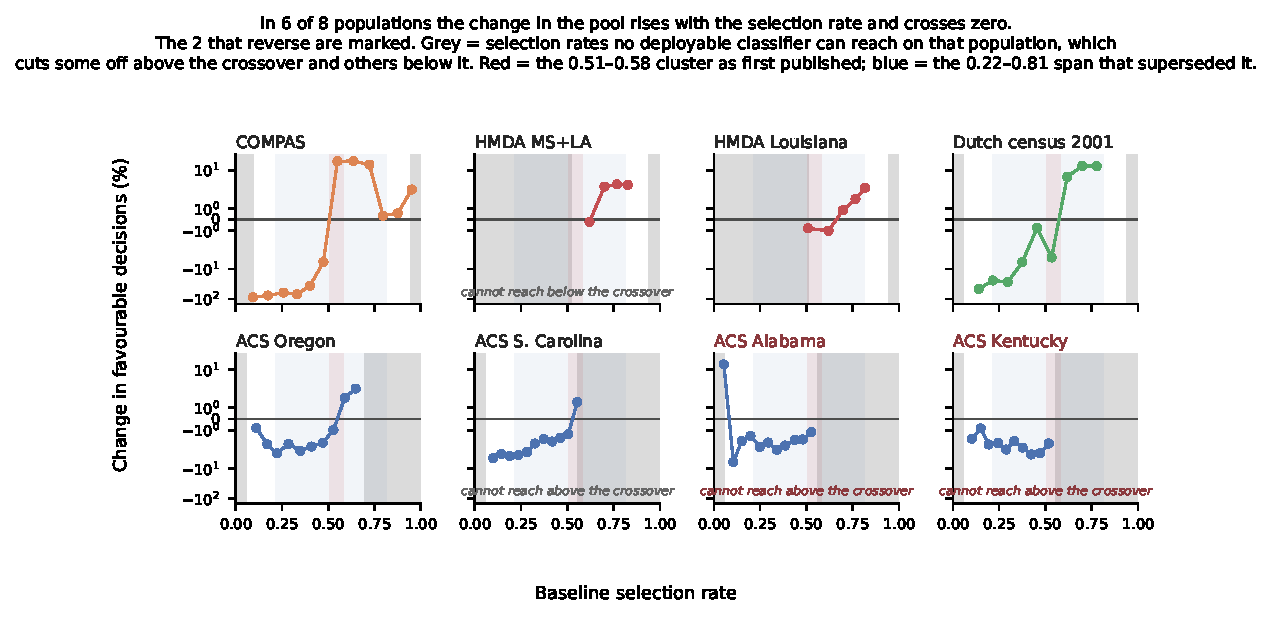
\includegraphics[width=\textwidth]{fig-crossover.pdf}
\caption{Every retained arm from every densely swept population. Within a population the
change in the pool rises with the baseline selection rate and crosses zero; the two that
reverse are marked, and both are sweeps whose viable band confines them below the crossover.
Panels are deliberately \emph{not} pooled: no pooled slope survives its pre-registered bar,
so one scatter would assert a common curve the data reject. Vertical band: the point-estimate
cluster of Table~\ref{tab:crossover}, drawn as first published;
Section~\ref{sec:boundaries} gives its later history.}
\label{fig:crossover}
\end{figure*}


\subsection{A single-factor design}

ACS Income's label is ``earns more than \$50{,}000'', and that threshold is a benchmark
convention rather than a fact about the world, which makes it a knob we can turn. Moving it
on one fixed state varies the selection rate while the sampled people, instrument,
feature set and group ratio stay fixed --- though moving the label redefines the
prediction problem itself, so this is one arm of the two-routes triangulation below, not
an isolation of the rate on its own. The change in the pool rises with the
baseline selection rate at $r = +0.801$ over four arms --- too few points for formal
inference, and reported as descriptive; a partial correlation on four points has one
degree of freedom and is omitted as uninformative. The sign flip is the substantive
observation: 22 decisions are destroyed per one created at a rate of 0.03, compared with
0.75 at 0.89.

\subsection{The transition appears without being manufactured}

The same transition also appears where nothing is manipulated at all. Pooling two states
across five real loan products, home improvement at a selection rate of 0.555 levels
\emph{down} ($-1.57\%$) while refinancing at 0.871 levels \emph{up} ($+2.95\%$), with
$r = +0.803$ and Spearman $\rho = +0.900$. This means a bank running one constraint across
its loan book would take opportunities away in one product while handing them out in
another, and its fairness report would show success in both.

\subsection{It is the rate, not the difficulty of the task}
\label{sec:tworoutes-note}

\begin{figure*}[t]
\centering
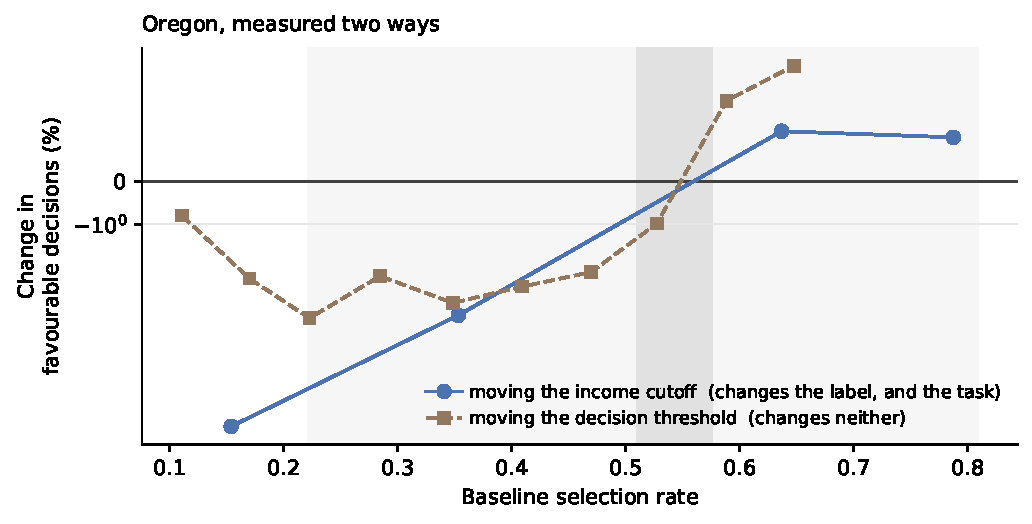
\includegraphics[width=0.86\textwidth]{fig-two-routes.pdf}
\caption{The design that separates the selection rate from the difficulty of the task. Moving
the income cutoff changes the label, and therefore how hard the problem is; moving the decision
threshold changes neither, only where the fitted model draws its line. Both routes cross zero
inside the same band. If difficulty were doing the work, the second curve would not reproduce
the first.}
\label{fig:tworoutes}
\end{figure*}


The design above moves the \emph{label}. ``Earns over \$100{,}000'' is not a rarer version of
``earns over \$20{,}000''; it is a harder problem. That design therefore cannot separate two
explanations which predict everything observed so far.

We separate them by holding the task completely fixed --- same rows, features, groups and
\emph{fitted scores} --- and moving only where the model draws its line. The relationship
reproduces, and so does the crossover's location: on Oregon the two routes give 0.362--0.653
and 0.353--0.637 (Fig.~\ref{fig:tworoutes}). \textbf{Task difficulty is not doing the work.}

With twelve points chosen from each population's viable band, the relationship holds on the
Dutch census ($+0.946$), South Carolina ($+0.905$) and COMPAS ($+0.844$). Alabama and Kentucky
return \emph{negative} values on eleven and ten arms; their viable bands top out at 0.566 and
0.561, at or below every crossover measured, so both sweeps lie almost entirely on one side of
the transition. \textbf{We therefore claim the relationship across the crossover and withdraw
any claim that it holds within the low-rate region alone.}

\subsection{Five domains, and the group-gap alternative}

\begin{table}[t]
\caption{The relationship across instruments, not pooled across them, for the reason
Fig.~\ref{fig:crossover} does not pool. This table's job is \emph{breadth} --- one population
per instrument, on whatever arms that population naturally supplies --- so the four-to-six-arm
correlations are descriptive, exactly as Section~\ref{sec:tworoutes-note} concedes for Alabama.
The dense-sweep columns carry the weight where a viable band allows twelve points, but
those twelve are thresholds applied to one fitted score vector on one sample and are not
twelve independent observations, so we quote no $p$-value on them: a Pearson test there
describes whether a sweep is monotone, not whether the rate predicts across populations. The
pre-registered alternative is refuted on the dense columns, not the sparse ones.}
\label{tab:domains}
\centering
\scriptsize
\setlength{\tabcolsep}{2.5pt}
\begin{tabular}{@{}lllcccc@{}}
\toprule
& & & \multicolumn{2}{c}{\textbf{natural arms}} & \multicolumn{2}{c}{\textbf{dense sweep}} \\
\cmidrule(lr){4-5}\cmidrule(lr){6-7}
\textbf{Instrument} & \textbf{Domain} & \textbf{Population} & \textbf{$r$} & \textbf{n} &
\textbf{$r$} & \textbf{n} \\
\midrule
ACS Income & income & Alabama & $+0.801$ & 4 & --- & --- \\
ACS Income & income & S. Carolina & --- & --- & $+0.905$ & 12 \\
HMDA & mortgages & MS+LA pooled & $+0.858$ & 4 & --- & --- \\
COMPAS & crim. justice & race arm & $+0.870$ & 5 & $+0.844$ & 12 \\
Dutch census & occupation & sex arm & $+0.915$ & 6 & $+0.946$ & 12 \\
LSAC & legal educ. & --- & unsweepable & --- & --- & --- \\
\bottomrule
\end{tabular}
\end{table}

Fig.~\ref{fig:crossover} shows every arm, and Table~\ref{tab:domains} the summary. The
pre-registered alternative --- ``this is a property of income prediction and American mortgage
lending'', requiring $|r| < 0.30$ --- is refuted on both new instruments, and refuted on their \emph{densely swept} arms rather than their sparse ones: COMPAS gives
$+0.844$ and the Dutch census $+0.946$ over twelve points each. Earlier versions of this paper
attached $p < 0.001$ to those coefficients; we withdraw it. Twelve thresholds on one fitted
score vector over one sample are near-deterministic transformations of each other, so the
Pearson null is the wrong reference and the effective sample size for a claim about
\emph{populations} is one. The population-level statistic this design supports is much
weaker: across the six densely swept populations the within-population slope is positive in
four and negative in two, a sign test at $p = 0.34$. We report it because it is the honest
number, and note that the two negatives are the sweeps Section~\ref{sec:tworoutes-note}
withdraws for sitting entirely below their crossover --- which is a stated exclusion, not a
rescue, and either way the prospective evidence for this paper lives in the sealed forecasts
and not in these coefficients. The four- and five-arm rows are reported for breadth and carry
no inferential weight on their own.

The oldest competing account is that the \emph{gap between groups} drives the direction. The
Dutch census has a gap of 0.298, roughly twice Adult's, making it the population where that
explanation should win. It gives $r = +0.915$ across all six arms, none excluded.

Because the parity-gap floor was tuned in-sample (Section~\ref{sec:setup}), the
\emph{natural-arm} column of Table~\ref{tab:domains} was re-scored at floors
0.02/0.05/0.08/0.10: each of those correlations stays between $+0.80$ and $+0.92$ with no sign
change at any floor (HMDA is floor-invariant outright; Alabama thins to two arms only at
0.10). \textbf{The dense-sweep column is a different matter, and an earlier version of this
paper claimed otherwise.} Table~\ref{tab:sensitivity}'s 0.05 column \emph{is} that dense-sweep
column, and one of its three entries is strongly floor-dependent: South Carolina reads
$+0.905$ at the committed floor and $+0.012$ at 0.02 and 0.01. So the floor is doing real work
on a number this paper leans on, and the correct statement is the narrower one --- the
natural-arm evidence is floor-robust, the dense-sweep evidence is not uniformly so, and South
Carolina's twelve-point correlation should be read as conditional on the exclusion rule rather
than as independent of it.

\subsection{Robustness}

\begin{table}[t]
\caption{What each manipulation preserves}
\label{tab:robust}
\centering
\small
\begin{tabular}{@{}lll@{}}
\toprule
\textbf{Manipulation} & \textbf{Direction} & \textbf{Magnitude} \\
\midrule
Route to the rate & unchanged & differs $3\times$ \\
Tolerance, $25\times$ range & unchanged & differs $4\times$ \\
Boosted trees (5/5 pops.) & unchanged & differs $3\times$ \\
Attribute, sex $\rightarrow$ race & unchanged & --- \\
Criterion $\rightarrow$ equalized odds & weaker, unevenly & differs $8\times$ \\
Optimiser $\rightarrow$ post-proc. & \textbf{vanishes} & --- \\
\bottomrule
\end{tabular}
\end{table}

Table~\ref{tab:robust} summarises. \textbf{Within a population, and in the attribute-blind regime, the selection rate
predicts which way and orders how much. Neither transfers between populations}: the signed distance from a
population's own crossover gives $\rho$ of $+0.96$, $+0.95$ and $+0.78$ in three of four
populations, but a pooled slope reaches only $r = +0.487$ against a pre-registered $+0.70$ bar.

\section{The Regime Boundary}
\label{sec:regime}

The relationship stops where the optimizer family changes, not where the protected attribute
becomes readable, and a sealed test with both readings' bars committed in advance is what
separates those. Under group-threshold post-processing \cite{hardt2016}, at each population's
natural operating point, the rate carries no information about the pool's direction
($r = -0.024$, against $+0.585$ for the reduction on the same populations); our pre-registered
prediction that the rule would carry over is a recorded failure. The missing cell decides
between the two available explanations: given the attribute under the \emph{same}
in-processing optimizer, the relationship survives at $r = +0.672$ across thirteen natural
arms --- the method reading, not the blindness reading. Two cautions we would rather state
than have computed for us: at thirteen arms the interval on that coefficient is wide enough to
touch the competing reading's region, and its difference from $+0.585$ is not itself a
difference. What carries more weight than either coefficient is the mechanism the failure
exposed --- the post-processor re-derives its own thresholds and returned an identical model
at all six operating points, so the measured effect was a constant divided by a shrinking
baseline.

\textbf{The theory's group-level claim is untouched.} Where the attribute is readable the
advantaged group loses and the disadvantaged gains, without exception across our
attribute-aware arms. That is a consistency check against a published theorem rather than a
forecast --- the theorem made the prior close to one --- and it separates cleanly from the
pool question: the theorem fixes each \emph{group's} direction wherever the attribute is
readable, while the \emph{pool's} direction, the sum it does not constrain, stays
rate-predictable under in-processing in both regimes and unpredictable only under
post-processing. A percentile-relaxed form of the theory's ordering agrees with the measured
direction on 24 of 26 arms and tracks our predictor at $r = +0.935$, so the selection rate is
a cheap proxy for a quantity the theory states expensively; the exact conditions were
certified on none of the 26 by our plug-in estimator, whose ratio diverges in the $\hat\nu$
tail, and we tried no other.

\section{Boundaries}
\label{sec:boundaries}

\subsection{Where the crossover sits, and what it cost to find out}
\label{sec:boundaries}

\begin{table}[t]
\caption{Crossover locations, with the existence of a crossing separated from its
location. \textbf{P(crossing)} is the share of nested rows-by-seeds resamples in which a sign
change can be bracketed at all; \textbf{crossover} is the median location \emph{conditional}
on one existing. Separating them is not pedantry: read under seeds only, the Dutch census
appeared to cross at 0.576 with a 95\% interval of 0.572--0.580 --- an apparently precise
estimate --- while under the nested bootstrap \emph{no} resample brackets a crossing, and the
published figure was a property of the six arms that produced it. An interval conditioned on
an event that may not occur cannot be read as an interval. The bracket-only rows assume a
crossing rather than estimating whether there is one, and the lending rows are point estimates
with no resampling; both are labelled as such rather than sharing a column with the nested
figures. The rates are not one economic object: survey rows are predicted-status rates over
sampled persons, lending rows are approval rates conditional on having applied, and COMPAS
inverts a risk score.}
\label{tab:crossover}
\centering
\scriptsize
\setlength{\tabcolsep}{2pt}
\begin{tabular}{@{}llccl@{}}
\toprule
\textbf{Population} & \textbf{Domain} & \textbf{P(crossing)} &
\textbf{Crossover} & \textbf{Uncertainty} \\
 & & & \textbf{\emph{given} one} & \\
\midrule
\multicolumn{5}{@{}l}{\emph{Nested rows-by-seeds bootstrap, 1{,}000 pairs}} \\
COMPAS & crim. justice & 100\% & 0.457 & 0.433--0.539 \\
S. Carolina & income & 97\% & 0.525 & 0.454--0.537 \\
Oregon & income & 99\% & 0.532 & 0.514--0.604 \\
Dutch census & occupation & \textbf{0\%} & --- & none crosses \\
\midrule
\multicolumn{5}{@{}l}{\emph{Bracket only --- crossing assumed, not estimated}} \\
Florida & income & --- & \textbf{0.284} & 0.259--0.309 \\
Ohio & income & --- & 0.556 & 0.528--0.585 \\
Pennsylvania & income & --- & \textbf{0.652} & 0.624--0.681 \\
\midrule
\multicolumn{5}{@{}l}{\emph{Lending --- one market, three overlapping estimates}} \\
HMDA pooled & mortgages & --- & 0.660 & point only \\
HMDA Louisiana & mortgages & --- & 0.659 & point only \\
HMDA refinance & mortgages & --- & 0.758 & point only \\
\bottomrule
\end{tabular}
\end{table}

The crossover was first published as a cluster, on four populations of one instrument. It did
not survive measurement. \textbf{Located crossovers span 0.22 to 0.81} --- 0.22 to 0.65 across
the ACS income sweeps, with the law-school and South Carolina mortgage brackets above 0.80 ---
so the location is population-specific and only sometimes near the middle. Nothing in this work
predicts it: the sealed test of the two candidate predictors returned \textsc{underpowered}
with three crossovers located against a floor of six, and three of ten large states have no
crossover to locate at all, sweeping U-shaped or levelling up throughout. The lending
estimates come from one two-state market read three overlapping ways, so ``lending is
different'' remains a hypothesis rather than a finding.

That history is the case for measuring rather than transporting, and it is made by the prior's
own failures rather than against them. Sweeping the arms where a fixed 0.54 fails shows they
are populations with no directional rule to get right --- non-monotone or outright inverted,
including one the rule scored \emph{correct}, whose correctness was therefore luck. A prior
read off a dashboard cannot detect that, because detecting it requires the sweep the prior
exists to avoid. The audit refuses all of them; only the prior is exposed.

\subsection{The procedure is unusable on very generous tasks}

Varying the selection rate by moving a threshold works by \emph{degrading} the classifier. On a
task where most people already qualify, reaching a low selection rate requires a model that
refuses qualified people, and past a point that model is worse than a constant. Defining the
\emph{viable band} as the range of selection rates reachable by a classifier still beating
$\max(p, 1-p)$: Dutch spans 0.895, COMPAS 0.859, typical ACS $\approx 0.51$, and LSAC only
\textbf{0.056}. On LSAC, where 89\% pass the bar, no choice of thresholds produces a usable
sweep. This is computable before running anything.

When the viable band forbids a sweep, the crossover can still be located by comparing natural
sub-populations --- which is how the mortgage crossover was first found.

\subsection{A sealed prediction, and what it cost}
\label{sec:sealed}

\begin{table}[t]
\caption{Sensitivity to the parity-gap exclusion. Correlation per population as the
threshold is loosened.}
\label{tab:sensitivity}
\centering
\footnotesize
\setlength{\tabcolsep}{5pt}
\begin{tabular}{@{}lcccc@{}}
\toprule
\textbf{Population} & \textbf{0.01} & \textbf{0.02} & \textbf{0.05} & \textbf{0.10} \\
\midrule
Dutch census & $+0.851$ & $+0.908$ & $+0.946$ & $+0.938$ \\
COMPAS & $+0.844$ & $+0.844$ & $+0.844$ & $+0.871$ \\
S. Carolina & $+0.012$ & $+0.012$ & $+0.905$ & $+0.849$ \\
Oregon & $+0.095$ & $+0.095$ & $+0.664$ & --- \\
Alabama & $-0.368$ & $-0.368$ & $-0.368$ & $+0.296$ \\
Kentucky & $-0.590$ & $-0.590$ & $-0.654$ & --- \\
\bottomrule
\end{tabular}
\end{table}

Every result above is a correlation computed after the arms were run, which is the weakest
support for a claim of the form \emph{you can know in advance}. We therefore ran the strongest
format available: nine populations whose direction had never been measured, with the rule, the
populations and the pass mark committed before any of them existed. Eight enter the sealed
score; the ninth, Taiwan, was sealed alongside them but registered as reported separately,
because a single non-Western population can carry no claim on its own (it was predicted
correctly: rate 0.885, observed $+0.68\%$).

\textbf{It failed. Four of eight, against a bar of seven, not beating a constant}
(Table~\ref{tab:sealed}).

\begin{table}[t]
\caption{The sealed prediction. Populations never previously measured; predictions committed
before the runs.}
\label{tab:sealed}
\centering
\footnotesize
\setlength{\tabcolsep}{4pt}
\begin{tabular}{@{}lrrcc@{}}
\toprule
\textbf{Population} & \textbf{Rate} & \textbf{$\Delta$pool} & \textbf{Pred.} & \textbf{Actual} \\
\midrule
MO, \$100k & 0.026 & $-16.48\%$ & up & \textbf{down} \\
AZ, \$100k & 0.037 & $-23.34\%$ & up & \textbf{down} \\
IN, \$70k & 0.081 & $-23.32\%$ & up & \textbf{down} \\
TN, \$50k & 0.255 & $-1.68\%$ & down & down \\
MD, \$50k & 0.508 & $+0.78\%$ & down & \textbf{up} \\
MI, \$30k & 0.612 & $+0.85\%$ & up & up \\
NC, \$20k & 0.789 & $+0.16\%$ & up & up \\
GA, \$10k & 0.905 & $+0.30\%$ & up & up \\
\midrule
Taiwan 2005 & 0.885 & $+0.68\%$ & up & up \\
\bottomrule
\end{tabular}
\end{table}

\textbf{What failed is a refinement, not the rule.} Table~\ref{tab:sensitivity} shows the
exclusion threshold doing real work: South Carolina moves from $+0.905$ to $+0.012$ when it is
loosened. Investigating that, we found the newly admitted arms are not noise --- at twenty
seeds they are consistently \emph{positive}, $+8.73$, $+6.85$, $+9.09$, six standard errors
from zero --- and concluded the relationship turns back up below a selection rate of 0.10. The
sealed rule carried that refinement.

All three held-out low-rate arms came out strongly \emph{negative}. Scoring the same eight arms
under the simpler rule we held before the refinement --- down below the crossover, up above it
--- gives \textbf{seven of eight}, its only miss being Maryland at 0.508, within 0.032 of the
crossover on an effect of $+0.78\%$. That seven is post-hoc and we do not claim it; what was
sealed scored four.

\textbf{The refinement was route-specific.} Its arms reach a rate near 0.05 by thresholding one
fixed score vector; the sealed arms reach it with a genuinely rarer label. At that rate the two
disagree completely, $+8.73$, $+6.85$, $+9.09$ against $-16.48$, $-23.34$, $-23.32$. So
Section~\ref{sec:tworoutes-note} qualifies: the two routes agree through the middle of the range
and diverge at the bottom, and the accuracy rule does not catch the divergent arms --- they
clear the trivial-predictor bar and remain artifacts.

A refinement drawn from four in-sample populations, internally consistent and backed by a
twenty-seed replication, made the prediction worse than the rule it replaced and no better than
a constant. Nothing in the in-sample data could have shown that.

\subsection{The rule re-sealed, and it holds}
\label{sec:resealed}

\begin{table}[t]
\caption{The re-sealed prediction: the unrefined rule --- down below 0.54, up at or above ---
committed before ten never-measured states ran. Bar: 9 of 10 \emph{and} beat the best
constant.}
\label{tab:resealed}
\centering
\footnotesize
\setlength{\tabcolsep}{4pt}
\begin{tabular}{@{}lrrcc@{}}
\toprule
\textbf{Population} & \textbf{Rate} & \textbf{$\Delta$pool} & \textbf{Pred.} & \textbf{Actual} \\
\midrule
NE, \$100k & 0.014 & $-6.35\%$ & down & down \\
AR, \$50k & 0.195 & $-2.55\%$ & down & down \\
OK, \$50k & 0.220 & $-12.78\%$ & down & down \\
WA, \$70k & 0.233 & $-5.52\%$ & down & down \\
NV, \$50k & 0.297 & $-1.57\%$ & down & down \\
MN, \$30k & 0.699 & $-0.04\%$ & up & \textbf{down} \\
CO, \$30k & 0.701 & $+0.63\%$ & up & up \\
KS, \$20k & 0.767 & $+0.58\%$ & up & up \\
WI, \$20k & 0.814 & $+0.69\%$ & up & up \\
IA, \$10k & 0.896 & $+0.04\%$ & up & up \\
\bottomrule
\end{tabular}
\end{table}

The unrefined rule --- down below 0.54, up at or above --- was committed with its ten
populations and its pass mark before any of their arms existed: at least 9 of 10 correct
\emph{and} strictly beating the best constant. \textbf{It holds: 9 of 10, best constant 6}
(Table~\ref{tab:resealed}). The re-seal applies none of this paper's tuned guards and scores
all ten populations raw, so it has nowhere to hide an exclusion, which makes it the cleanest
scoring here.

Two statistics, because they answer different questions and the weaker one is the honest
headline. A guesser at the constant's rate reaches 9 or more with probability $0.046$. But
rule and constant disagree on only five arms, the rule wins four of those five, and the
one-sided sign test on the discordant calls gives $p \approx 0.19$. Nor is this the first
sealed attempt at a direction rule, so the binomial tail carries a sequential correction whose
size is a judgement we should not make in our own favour: read narrowly it is a factor of two
and the tail is near $0.09$; read as this paper's own abstract counts them --- nine sealed or
registered direction tests --- it is a factor of nine and the tail is $0.41$. Across the
conventional line either way, and not close to it on the wider reading.

\textbf{What the pass cannot establish, stated where the score is.} Every arm reaches its rate
by the income-cutoff route, and the achieved rates leave the interior of $(0.30, 0.70)$
unsampled --- the nearest sit at $0.297$, $0.699$ and $0.701$. So the pass cannot separate the
selection rate from label rarity as the operative variable, nor the value $0.54$ from any
prior in that interval: \textbf{a rule reading only the income cutoff scores identically
here}. The screen-gated race cohort was registered to break exactly this confound and did, on
mixed-route arms off-instrument and off-continent, where the cutoff-only null scored 5 of 10
against the rate rules' 8--9 --- ten arms from two person-samples, so the confound breaks
within populations rather than across them. Its sealed S1 nonetheless \emph{fails} by its own
letter, because a $0.50$ prior edged the $0.54$ prior 9 to 8: the rate carries the prediction
and the specific value does not.

\textbf{The paired statistic has a ceiling this design cannot raise.} A third cohort was built
to supply the discordant arms the sign test needs, and its pre-committed magnitude guard
removed ten of twenty-four --- removing them \emph{near the crossover}, because effect size
grows with distance from it ($r = +0.648$). Four discordant arms survived, the rule won all
four, and four of four is $p = 0.0625$: the bar was arithmetically unreachable. The guard and
the discordance a paired test needs are anti-correlated by construction, so the weakness does
not yield to a larger balanced cohort. On a second, post-hoc cohort of larger states the fixed
prior scored 5 of 10, and every miss agrees with that state's own measured crossover ---
which is the case for measuring rather than transporting, made by the prior's failures.

\subsection{Small populations}

Below roughly 2{,}500 test subjects the method's own randomness exceeds the entire effect of
the constraint. This is a specific instance of predictive multiplicity
\cite{black2022,long2023} --- and Long \emph{et al.} \cite{long2023} show fairness
interventions themselves exacerbate it ---
models with equivalent aggregate performance disagreeing substantially on individuals --- and
we position it as a caution supported by that literature rather than as a novel finding. COMPAS has 1{,}584 and flips sign between seeds on two of four arms; LSAC has
6{,}240 and flips on none. COMPAS carries direction here and never magnitude.

\subsection{How the withdrawal is implemented: a lottery}
\label{sec:lottery}

At severely cut operating points the fitted mixture stops being a graded adjustment and
becomes a lottery: nobody below the threshold receives any probability, and every predicted
positive of both groups is kept at one flat rate --- 0.65 on the Dutch census arm, 0.135 on
COMPAS --- with keep probability uncorrelated with the person's own score. The gap closes by
random discard and the certificate is unchanged, which matters because a model that cannot
generate a truthful individualized reason for a denial sits badly with adverse-action and
notice duties. \textbf{It is a checkable hazard rather than a cost of parity}: a control at
each population's natural operating point finds every mixture graded, so the signature belongs
to constraints pushed to extremes and not to withdrawal as such --- which is why Algorithm~1
probes for it (line 19) and why the full treatment, including the search of a richer
two-threshold class that returns an empty feasible set, is reported separately.

\section{The Audit: Give, Take, or Refuse}
\label{sec:procedure}

Algorithm~\ref{alg:locate} states the procedure. Three of its steps are worth drawing out,
because each is a place where a plausible-looking run returns a meaningless answer.

\textbf{It can refuse.} Lines 6--8 compute the viable band and exit before any constraint is
fitted, if no threshold reaches a low selection rate with a model still beating the trivial
predictor. On LSAC that band is too narrow to sweep (Section~\ref{sec:boundaries}) and the procedure
declines, rather than returning arms that would be discarded later.

\textbf{It can return \textsc{void}.} Line 16 requires enough arms to survive the guards
and the pool to have moved at all. A
correlation computed over arms that barely move is fitted to noise: Connecticut returns
$r=-0.924$ on a spread of a tenth of a percentage point, and without this test that number
reads as a refutation of the whole finding.

\textbf{It can return \textsc{non-monotone}, and on current data it often will.} Lines
20--22 exist because the assumption behind bracketing --- one rising sign change --- is
itself population-dependent: among the ten largest states we swept, three are U-shaped
and the 2022 vintages at nominal labels invert, so a bracket step that assumed
monotonicity would return a confident wrong direction precisely there. A
\textsc{non-monotone} verdict means the directional rule does not apply to this system,
which is a first-class answer, not a failure of the audit. A sweep whose retained arms
all share one sign is the opposite case and returns that direction (line 24): the
constraint moves the pool the same way across the whole viable band, which is what
``levels up throughout'' means operationally. Two cautions the earlier version of this
algorithm kept in prose are now steps: arms below a selection rate of $0.10$ are marked
\emph{advisory} and excluded from the shape call (line 14), because below that boundary
the two routes to a rate give opposite signs (Section~\ref{sec:boundaries}) and the
accuracy guard does not catch it; and every fitted arm is probed for the flat
keep-probability signature (line 19), because a lottery under the certificate is a
finding the direction verdict alone would hide. The probe's decision rule, stated so it
can be implemented: flag an arm whose mean granted probability just below the boundary
is under 0.10 while the keep-probability's correlation with the score above it is
$\approx 0$ --- the observed separation is wide (0.00--0.07 against 0.17--0.43, and
$\approx 0$ against $+0.37$ to $+0.73$).

\textbf{Guard provenance, in one place.} A guard's provenance belongs to the pair it forms
with a result, not to the guard. The band span, the parity-gap floor and the threshold grid
are exploratory, fixed in the threshold sweep's own pre-registration and confirmatory for
every seal after it. Three are not. The 2-point void guard was written for the equalized-odds
pre-registration and imported \emph{backwards} into the threshold sweep, moving three arm sets
from refutation to \textsc{void} --- a change in the conjecture's favour, against which the
same audit found no arm set that passed on noise. The 0.10 advisory boundary postdates the
sweep it is applied to and descends from a clause that was sealed, scored 4 of 8 and
withdrawn; it survives only where it can refuse an arm but not manufacture a correct call. And
the 2,500 noise floor is the one this paper's own drafting got wrong: dated from the constant
carrying it today it looks retrospective, and dated from its value it is exploratory, fixed
before the sweeps and frozen in every seal since.

\textbf{It can return \textsc{indeterminate}.} Lines 28--29 refuse a sign call when the
deployed rate sits inside the located bracket, or when the nearest arms' effects are
within seed noise --- precisely the two conditions under which this project's own record
shows a sign call has nothing to grip: Maryland's miss sat at the cluster's edge
(Section~\ref{sec:sealed}), and Minnesota's was an effect of $-0.04\%$ that flips sign
across seeds. The registered
rubric of the re-seal did not have this verdict and was charged a miss for it; the
algorithm inherits the lesson.

\textbf{The magnitude guard is measured, not assumed.} Line 28's refusal rests on the
claim that a near-zero effect has no sign to predict. Two sealed cohorts run after this
algorithm was written put a number on it: across their forty arms the rule is correct on
\textbf{21 of 22} arms whose effect exceeds one point and on \textbf{11 of 18} below it ---
95\% against 61\%, which is a coin flip. Those arms span 19 and 15 disjoint person-samples,
and clustering on the sample rather than the arm leaves the split intact: 85--100\% above
the threshold against 37--82\% below, intervals that barely meet.

\textbf{What that measures is the floor's existence, not its location.} The two read alike
and they are not the same claim, so we separate them. Sweeping the guard over the same forty
sealed arms, \emph{every} value from 0.25 to 5.00 points separates the reliable arms from the
unreliable ones, by between 13 and 35 percentage points; the largest separation is at 0.25
($+35$) and the committed 1.0 gives $+34$. A dip to $+13$ at 0.75 shows the estimate is noisy
at forty arms, which is the useful part: no value in the range can be argued to be the right
one. The guard's \emph{existence} is therefore measured, and its \emph{value} is
operational --- a round number fixed in the third cohort's protocol before its arms existed,
which the data neither singles out nor contradicts. The cohorts were scored at 1.0 exactly as
pre-registered; the sweep is post-hoc and re-scores nothing.

\textbf{It returns a sign, never a size.} The distance from the crossover \emph{orders} the
effect within a population, so a team can rank its own segments; but no slope transfers between
populations, so lines 32 and 34 return a direction and stop there.

\textbf{What it is for, and what it is not.} The audit applies where the pool of
favourable decisions can actually change size. Where the allocation is
capacity-pinned --- a fixed number of seats, beds, or slots --- the total is constant
by construction, the directional quantity this paper measures cannot arise, and the
audit is out of scope from line~0; this is the fixed-resource regime of
\cite{goethals2024}, and clinical triage and admission commonly live there. No
natural operating point below 0.13 has been probed in this record, so deployed rates
below that carry an untested-region caution on top of every verdict.

\textbf{What it needs, and what it costs.} The audit requires a held-out sample carrying
the protected attribute: audit-time access to $a$, which is legally and practically
distinct from decision-time use and is the regime bias-testing provisions contemplate
(Section~\ref{sec:scope}) --- in US credit, the self-test privilege of Regulation~B
(12~CFR~\S1002.15) exists for exactly this, though it is conditional: the privilege
attaches to a lender's own voluntary self-test and expects appropriate corrective
action, and an analysis of public HMDA records, like this paper's, is not itself a
privileged self-test. It fits the constraint $12 \times \mathrm{seeds}$ times; with five seeds
and the linear learners used here, one fit takes 2--10 seconds at $15$k--$69$k training
rows (measured on a laptop CPU), so a full audit is minutes per population, and its cost
scales linearly in the base learner's own fit time since each reduction call is a
sequence of learner refits. A cheap pre-screen exists: the relaxed-$\zeta$ ordering of
Section~\ref{sec:regime} needs no constraint fits and correlates with the predictor at
$r=+0.935$.

\textbf{What the sweep buys that one fit does not.} A team able to run $12 \times$ seeds
constrained fits could instead run \emph{one}, at the operating point it already uses, and
read the pool change off it --- so what has prediction bought over measurement? A single fit
returns a point; the sweep returns a neighbourhood. Two measurements separate them. Across 639
adjacent arm pairs whose effects both clear the 1.0-point guard, 69 --- 11\% --- disagree on
the \emph{sign}, so the direction one fit reports is not reliably a property of the population
rather than of the threshold that fit happened to use. And populations sit close to their own
boundary: of 21 disjoint person samples carrying both a located crossover and a natural arm,
11 sit within 0.10 of the crossover and 6 within 0.05, Florida 2018 sitting 0.004 from it. For
those teams the direction is not a fact to accept or refuse but a threshold they already
control, and one fit reports the withdrawal without reporting the lever. That the crossover
cannot be looked up rather than measured shows in the same set: Florida enters twice, once per
attribute, crossing at 0.284 read by sex and 0.439 read by race --- the same people, two
boundaries.

The limit belongs with the answer. The sweep does not buy a better estimate of what the
constraint does at today's threshold; repeated fits at one point buy that. What it buys is
\emph{shape}. Five of the 21 sit more than 0.20 from their crossover and would have decided
the same from one fit --- and that 24\% over-states the waste, because every sample in the set
has already passed the monotonicity screen, and the 22\% admitting no rule never enter it. A
team cannot learn which group it is in without running the sweep, which is the reply in one
line: the audit is not circular, because its output is not the quantity a single fit measures.

\textbf{What it actually returns, totalled.} Run over the 52 population-label pairs whose
stored sweeps resolve to a dataset spec --- fourteen further IPUMS sweeps are stored but
unmapped, and are excluded rather than guessed at --- the distribution
is: 29 directional verdicts (20 \textsc{withdrawal}, 9 \textsc{extension}), 8
\textsc{non-monotone}, 13 \textsc{void}, one refusal at the noise floor (COMPAS), and
one bracket with no natural arm to read against. Every one of the 29 directional
verdicts matches what the fitted constraint did at that population's natural operating
point --- a consistency check on the audit's reading of its own sweep, not independent
validation, since the natural arm is part of the curve being read. That distribution is computed over the sweeps this project happened to accumulate, which
were never randomly chosen, so it answers a question about this project rather than about
populations. A survey with a pre-committed frame answers the latter.

\textbf{The frame, since ``at random'' means nothing without one.} Every combination of the
fifty US states, the 2014, 2018 and 2019 ACS vintages, and the two protected attributes, with
the income cutoff held at \$50{,}000 --- 300 population-label pairs. The 2022 vintage is
excluded because its inversion is a diagnosed nominal-label artifact, and including it would
conflate a label problem with a landscape property. Fifty pairs were drawn uniformly at
random under a fixed seed, and the frame, the seed, the draw and the exclusion were all
committed to version control before any arm ran; the drawn list is in the repository. The
draw came out balanced without being forced: 25 of each attribute, and 14, 14 and 22 across
the three vintages. The fifty pairs span \textbf{48 disjoint person-samples}, two state-years
having been drawn under both attributes.

The result: \textbf{78\% admit a directional rule and 22\% do not}, of which 64\% are
classic single-crossing landscapes. Resampling \emph{populations} rather than draws puts the
directional share at 66--89\%, and leaving each population out in turn never moves it below
77\%. The convenience sample was mildly optimistic --- it implied 15\% non-monotone --- and
the larger number is the one to quote. The refusals are not
silences. A \textsc{void} arm is one whose pool change spans under two points across the
entire viable band --- median 1.47 --- which tells a deployer that the direction question is
\emph{moot} on their system, not that it is unanswerable; a \textsc{non-monotone} verdict
says the rule does not apply here, which is a finding about the system; and the noise-floor
refusal says the population is too small to audit at all. Counted that way, 48 of the 52
return something a team can act on and four return nothing --- three sweeps too thin to read
and one bracket with no natural arm. The honest summary: the audit gives a \emph{direction}
a little under six times in ten, tells a team the question is moot or the rule inapplicable
in most of the remainder, and is silent on four of fifty-two. Finally, an ex-ante verdict earns trust only if checked:
whatever the verdict, including refusals, the deployed system's measured pool change and
who-pays decomposition (Section~\ref{sec:whopays}) should be reported after the fact ---
the verdict is falsifiable at deployment, and Section~\ref{sec:discussion} makes this a
requirement rather than advice.

\textbf{The direction survives the extraction a deployer must apply.} Every direction
result above is measured on the randomized mixture, but a lender under
adverse-action-notice duties deploys a \emph{deterministic} model, so we tested the
extraction directly: thresholding the mixture's per-person probability at $0.5$ on the
natural arms of ten populations spanning both directions. The extracted model agrees
with the mixture's pool direction on \textbf{10 of 10}, with the parity repair largely
intact (extracted gaps $0.009$--$0.034$ against baseline gaps $0.08$--$0.19$). One
deployment fact surfaced on the way: an extraction that instead tries to reproduce the
mixture's own operating point cannot generally do so, because the mixture's probability
takes few discrete values and the ties force the deterministic threshold off the target
rate --- on three cutting populations far enough off to flip the sign of the measured
pool change. Thresholding at $0.5$ is the well-defined extraction, and it is the one
that preserves the verdict. The caveat composes with Section~\ref{sec:lottery}: these
are natural arms, where the mixture is graded; a flat-lottery arm has no
score-respecting extraction, and derandomizing it undoes the parity it bought.

\begin{algorithm}[t]
\caption{Directional audit: decide whether the predictor applies at all; if it does, locate
the crossover and decide whether to add a floor}
\label{alg:locate}
\begin{algorithmic}[1]
\REQUIRE deployed model $h$, held-out $(X,y,a)$ \emph{of the vintage to be deployed on},
fairness constraint $C$
\ENSURE predicted direction, and whether a selection-rate floor is needed
\IF{$C$ does not constrain selection rates}
  \RETURN \textsc{out of scope} \COMMENT{e.g.\ equalized odds}
\ENDIF
\STATE $\pi \leftarrow \max(\bar{y},\, 1-\bar{y})$ \COMMENT{trivial-predictor accuracy}
\STATE $s \leftarrow h(X)$
\STATE $\mathcal{V} \leftarrow \{\tau : \mathrm{acc}(s>\tau) \geq \pi \;\wedge\; 0.05 \leq
       \overline{(s>\tau)} \leq 0.95\}$
\IF{$\mathrm{span}(\mathcal{V}) < 0.40$}
  \RETURN \textsc{unsweepable}; compare natural sub-populations
\ENDIF
\STATE $T \leftarrow$ 12 thresholds from $\mathcal{V}$, spread evenly in \emph{selection rate}
\FORALL{$\tau \in T$}
  \STATE $r_\tau \leftarrow \overline{(s>\tau)}$; fit $C$ on the arm thresholded at $\tau$
  \STATE $\Delta_\tau \leftarrow$ \% change in favourable decisions
  \STATE discard $\tau$ if parity gap $<0.05$ or $\mathrm{acc}<\pi$; mark $\tau$
         \emph{advisory} if $r_\tau < 0.10$ \COMMENT{route-divergence region}
\ENDFOR
\IF{fewer than 4 non-advisory arms remain, \OR $\max\Delta - \min\Delta < 2$ points}
  \RETURN \textsc{void} \COMMENT{nothing moved; not a refutation}
\ENDIF
\STATE probe each fitted arm's mixture for a flat keep-probability
       (Sec.~\ref{sec:lottery}); flag any flat arm
\IF{$\mathrm{sign}(\Delta_\tau)$ changes more than once across the non-advisory arms,
    \OR changes from $+$ to $-$ as $r_\tau$ rises}
  \RETURN \textsc{non-monotone} \COMMENT{the rule does not apply here}
\ENDIF
\IF{every non-advisory $\Delta_\tau$ shares one sign}
  \RETURN that sign's verdict \COMMENT{it holds across the whole viable band}
\ENDIF
\STATE $c \leftarrow \big(\max\{r_\tau\!:\!\Delta_\tau<0\},\; \min\{r_\tau\!:\!\Delta_\tau>0\}\big)$
\STATE $r_0 \leftarrow$ selection rate of the deployed model
\IF{$\min c < r_0 < \max c$, \OR $|\Delta|$ at the arms nearest $r_0$ is within seed noise}
  \RETURN \textsc{indeterminate} \COMMENT{the sealed record's misses live here}
\ENDIF
\IF{$r_0 \leq \min c$}
  \RETURN \textsc{withdrawal}; add a selection-rate floor
\ELSE
  \RETURN \textsc{extension}; the floor buys little
\ENDIF
\end{algorithmic}
\end{algorithm}

The floor is \textbf{not a new method}: a selection-rate floor is a linear moment constraint
inside the framework of \cite{agarwal2018}, and a variant of the minimum rate constraints of
\cite{mittelstadt2023}. It costs about 0.12 accuracy points and moves the exchange rate from
1.47 favourable decisions destroyed per one created to 0.88 across nineteen arms, landing below
1.0 in sixteen of them, with the benefit scaling with the damage at $r \approx -0.99$ ---
sub-1.0 being a descriptive count of predicted labels, not a welfare verdict, per the
accounting caveat of Section~\ref{sec:whopays}; the group-conditional flows are what a
welfare reading would weigh. And because magnitude does not transfer across populations,
the floor is issued provisionally: the ex-post measurement the Discussion requires ---
the deployed system's pool change and who-pays decomposition, with and without the floor
--- is part of the prescription, not an optional follow-up.

\section{Method, and What We Got Wrong}
\label{sec:failures}

Table~\ref{tab:registered} is the complete ledger --- every registered or sealed test, with its
committed bar and its outcome, failures included and uncorrected. Counted once and
consistently it holds \textbf{eighteen} rows: twelve fail, three record a hold (one alongside
a failed first stage), two returned underpowered, and one settled a reading rather than a pass
or a fail. Of the nine that test a \emph{direction} rule on populations it had not seen, one
passed. The rows should not be read as eighteen attempts at one claim of which three
succeeded: each targeted a different claim, each failure removed a stronger claim than the one
that survives, and the last column records what each row settled. The failures are boundary
measurements; the passes are tests of the claim \emph{as those boundaries define it}.

Three episodes are worth stating in the body because each cost a claim the paper would
otherwise still be making. The rule does not survive equalized odds ($r = +0.334$ against a
$+0.70$ bar), which is why the claim reads \emph{parity} and not \emph{group fairness}: parity
controls approval rates directly and equalized odds does not. Our attempt to \emph{derive} the
rule was beaten by a constant, which is why the paper is empirical and says \emph{predicts}
rather than \emph{causes}. And a refinement drawn from four in-sample populations, internally
consistent and backed by a twenty-seed replication, was sealed, scored 4 of 8, and made the
prediction worse than the unrefined rule it replaced --- nothing in the in-sample data could
have shown that, which is the whole argument for sealing.

Two published results of our own are withdrawn here rather than quietly corrected: two
correlations previously reported at $+0.979$ and $+0.968$ are void, exposed by an exchange
rate of exactly $0.000$ --- the post-processor had returned an identical model at every
operating point, so the effect was a constant divided by a shrinking baseline. A published
crossover was also downgraded by a bootstrap we chose to run against our own result.



\begin{table}[t]
\caption{Every registered or sealed test. Each row targets a different claim; the last
column is what its outcome settled. Nothing is omitted.}
\label{tab:registered}
\centering
\scriptsize
\setlength{\tabcolsep}{3pt}
\begin{tabular}{@{}p{2.35cm}p{1.55cm}p{3.6cm}@{}}
\toprule
\textbf{Test} & \textbf{Bar / outcome} & \textbf{What it settled} \\
\midrule
HMDA sweep & 4 of 4; got 2 --- fail & our sweep procedure is unreliable on mortgage data,
so no claim rests on it there \\
EO transfer & $r \geq +0.70$; $+0.334$ --- fail & the rule works for parity, which controls
approval rates directly; it failed for equalized odds, which does not \\
Post-processing transfer & carry over; $r = -0.024$ --- fail & the rule stops where the
model may read the protected attribute --- the boundary of Sec.~\ref{sec:regime} \\
Derivation & beat a constant; beaten --- fail & our own attempt to derive the rule lost
to a constant; the first-order account we could not extend to the blind randomized case is
named in Sec.~\ref{sec:related} \\
Sealed rule, refined & 7 of 8; got 4 --- fail & the extra clause added from early data was
wrong, and is withdrawn \\
Attribute-aware consistency & 9 of 9; got 9 --- \textbf{holds} & where the attribute is
readable, the disadvantaged group always gains; a theory-consistency check run to a
pre-committed bar, not forecasting skill --- the theorem made the prior $\approx 1$ \\
Re-seal, unrefined rule & 9 of 10 + beat constant; got 9, constant 6 --- \textbf{holds} &
the simple rule predicts populations it has never seen, from the rate alone \\
Crossover residual & 6+ located, $\rho \geq 0.70$; 3 located --- underpowered & neither
candidate judged; a third of large states have no crossover to locate \\
Sealed magnitude model & beat predict-zero; MAE 4.50 v.\ 0.77 --- fail & size cannot be
predicted from distance and band span; the direction-only concession is earned \\
Sealed shape boundary & scored$-$1 + beat const.; 4 of 6 --- fail & the base-rate boundary
called every 2014 shape and both sealed flips; the 2022 inversion was since traced to
the label's sliding \emph{quantile} (see Limitations) \\
Sealed attribute-independence & scored$-$1 + beat const.; 2 of 6 --- fail & shape is not a
label-side property: every race arm is classic at tenfold the sex arms' signal, pointing
at gap size as the governing variable \\
Sealed cross-task shape & scored$-$1 + beat const.; 0 of 4 --- fail & the boundary does
not transfer to two non-income tasks; every scored call inverted --- transferred structure with a flipped sign, unexplained \\
Regime deconfounding & two sealed readings; R1 18/18, $r=+0.672$ --- method reading &
the pool boundary is the optimizer family, not blindness; the theorem's group
directions hold in every aware cell (Sec.~\ref{sec:regime}) \\
Six-market lending seal & M2: scored$-$1; 2 of 6 --- fail. M1: floor 4; 2 located ---
underpow. & the sweep is unreliable on mortgage data on six independent markets; the natural-arm direction holds 12 of 12 on the auditable arms of 40 markets, where a
constant ``up'' also scores 12 of 12; both
located midpoints sit at 0.80--0.85 \\
Third cohort (deconfounding) & S1 floor 12: 7 --- underpow.; S2 floor 2: 1; S3 floor
3: 0 & Brazil's sex gaps sit below the audit's own floor and the gates refused them;
Mexico 2015 brackets the first non-US crossover \\
Third direction cohort & 13/14 + beat const.\ + paired $p<0.05$; got 13, const 9,
$p=0.062$ --- fail & the paired statistic is not fixable by a balanced cohort: the
pre-stated magnitude guard deletes the near-crossover arms that discriminate
($r = +0.648$ between distance from the crossover and effect size), leaving four
discordant arms where four of four is already $p = 0.0625$ \\
Sealed lending cohort & 8/8 (5 pops.) + beat const.; const.\ also 8/8 --- fail &
the purpose-only null is beaten 8 vs 5: the loan product does not carry the prediction, the
measured rate does --- the first sealed evidence of this on real approvals rather than
predicted labels \\
Race cohort (screen-gated) & S1: 8/10, but 0.5-null 9 --- fail; S2 --- holds & the
cutoff null is beaten 8--9 vs 5: \textbf{it is the rate}, not label rarity; the 0.54
value holds no in-band privilege; within-population passes off-instrument at
$\rho \ge 0.9$ \\
\bottomrule
\end{tabular}
\end{table}

\section{Limitations}

\textbf{Most of the evidence is about predicted labels, not allocations.} In five of the eight
sources no one receives anything: ``favourable decisions'' are a classifier's labels over
people whose incomes, occupations or bar results already exist. HMDA is the one source
recording real allocative decisions --- and it is also where the direction reverses and where
our sweep protocol failed its held-out test, so whether the construct transports from
status-prediction benchmarks to allocation data is an open question rather than an assumption
we are entitled to. The practical advice of Section~\ref{sec:procedure} is addressed to teams
making real allocations, and they should read this paragraph first.

\textbf{The lending evidence is thinner than its market count suggests.} Forty markets carry a
rate-bearing arm on each attribute, but every one of the twenty-six sex arms falls below the
audit's own disparity floor --- median baseline gap 0.013 against the race arms' 0.079 --- so
the allocation result rests entirely on race arms. That is a property of US mortgage approval
rather than a gap in the method, and the audit refuses those arms correctly. Nor does either
lending count discriminate: every arm sits at a rate of 0.82 or above, so the rule predicts
extension on all of them and a constant scores identically. US mortgage approval supplies no
market whose rate straddles a crossover, so it cannot test the rule at all.

\textbf{Magnitude does not transfer} between populations, only within them, and a sealed model
of it lost to predicting zero. \textbf{The crossover's location is unexplained and wider than
it looked}: located values span 0.22 to 0.81, the sealed test of the two candidate predictors
returned underpowered, and some populations have no crossover to locate. \textbf{We cannot say
why the rule works.} Our own derivation lost to a constant; the first-order account we could
not extend to the blind randomized case is named in Section~\ref{sec:related}.

\textbf{A label is not a task.} A fixed nominal outcome definition is a different task each
vintage: a dollar cutoff slides down an inflated income distribution, and restoring the
earlier shape requires matching the label's \emph{quantile}, not its real price ---
CPI-anchoring is not enough. Four 2022 populations invert for this reason, and one 2014 state
inverts at a lower cutoff, so this is a property of nominal labels rather than of a vintage.

\textbf{Coverage} is eight data sources, five countries and two decades, of which 152 of 161
populations come from two instruments; the eight sources remain the honest count of
independent instruments. Taiwan, Brazil and Mexico are the non-Western populations and arrived
late enough that most of the record predates them. The only EU population is the 2001 Dutch
census, which by this paper's own vintage standard grounds no claim about current EU
deployments.

\section{Discussion}
\label{sec:discussion}

\textbf{What a practitioner can use.} Run the audit on your own data. It will locate your
crossover, tell you your system admits no directional rule, or tell you the question is moot
because the pool barely moves across your whole viable band --- and each of those is an
answer. Where it returns a direction and that direction is withdrawal, a selection-rate floor
is the remedy: not a new method, but a linear moment constraint inside the reductions
framework \cite{agarwal2018} and a variant of the minimum-rate constraints of
\cite{mittelstadt2023}. It costs about 0.12 accuracy points and moves the exchange rate from
1.47 destroyed per created to 0.88. Two honest consequences follow. Because the floor is that
cheap, a team that expects withdrawal and does not want to sweep should simply apply it; what
the audit adds is the ability to tell in advance whether it is needed, how far the operating
point sits from the sign change, and whether the population admits an answer at all. And
whatever the audit returns, the deployed system's pool change and who-pays decomposition
should be measured afterwards and reported beside the parity number --- so that escaping the
ex-ante audit buys no escape from the accounting.

\textbf{What to report.} The parity difference alone certifies both outcomes this paper
distinguishes. A report that adds the pool change and the group-conditional flows costs
nothing to compute, requires no doctrinal commitment, and is the difference between a
dashboard that can tell those outcomes apart and one that cannot.

\textbf{Adversarial inputs.} A procedure that can refuse can also be gamed, in four places we
can name: the label definition, the segmentation the audit is run over, the sweep's own
parameters, and refusal used as an exit. The countermeasures are symmetrical --- fix the
label's quantile rather than its nominal value, pre-register the segmentation, freeze the
sweep grid, and pair every verdict including a refusal with the ex-post accounting above. One
concrete instance is worth stating: on HMDA a single constraint earns ``extension'' on the
pooled book while concentrating withdrawal in home improvement, so a segmentation chosen after
the fact can hide the thing the audit exists to surface.

\textbf{What we are not claiming.} The rule is not surprising once stated --- say yes often and
the constraint tends to give, say yes rarely and it tends to take. What is not available
without measuring is where the boundary falls for a particular population, and located
crossovers span 0.22 to 0.81. In the one setting where we drew populations at random rather
than choosing them, no population's operating rate reached 0.55 and half of those with a
computable rate sat inside the band where an unaided reading of ``often'' against ``rarely''
has nothing to say. A further fifth follow no directional rule at all, and there the intuition
returns a confident answer while the audit declines to.

\section*{Appendix: Two Worked Traces of Algorithm 1}

\textbf{Oregon 2018, sex, to a verdict.} Demographic parity constrains selection rates:
in scope (line 1). Trivial-predictor accuracy $\pi = 0.636$ (line 4); the viable band
clears the 0.40 span bar, so the sweep proceeds (lines 6--9). The stored sweep holds 18
arms; the guards discard 2 on the parity-gap floor and 2 as worse than doing nothing,
leaving 14 spanning rates $0.111$--$0.653$, none below the 0.10 advisory boundary
(lines 11--15). Their pool changes span 7.14 points, clearing the void guard (line 16).
The signs, sorted by rate, are
\texttt{-{}-{}-{}-{}-{}-{}-{}-{}-{}-{}-{}+++}: one rising change, so the landscape is
monotone-crossing (lines 20--25) and the bracket is $c = (0.528, 0.589)$ (line 26). The
deployed model's rate is $r_0 = 0.353$ --- below $\min c$, outside seed noise: verdict
\textsc{withdrawal}, add a floor (line 32). What the constraint in fact does at Oregon's
natural arm: $-3.0\%$ of the pool.

\textbf{LSAC bar passage, to a refusal.} Trivial-predictor accuracy $\pi = 0.890$ ---
almost everyone passes. The viable band spans $0.056$, far under $0.40$: verdict
\textsc{unsweepable} at line 8, before a single constraint is fitted. Had the guard been
ignored, the stored sweep shows what awaited: five of seven arms fall below the trivial
predictor and the two survivors are too few to read --- \textsc{void}. Both endings
refuse; neither manufactures a direction.

\section*{Reproducibility}

Code, stored results and the full document trail are in the accompanying repository, which
holds the per-test registration and scoring commits, the OpenTimestamps receipts for the seals
that carry them, and the complete eighteen-row ledger. Every figure here is re-derived from
stored results by a test suite that fails if a documented number and its experiment disagree,
and counts appearing in more than one place are derived from one source and checked against
each other --- after an audit found four descriptions of the same table. One limit cannot be
repaired retroactively: for ten of the sixteen seals the ordering rests on git commit
timestamps from our own machine, which an outsider must take on trust. The later seals carry
external anchoring; the earlier ones do not.

\begin{thebibliography}{00}

\bibitem{agarwal2018} A. Agarwal, A. Beygelzimer, M. Dud\'{i}k, J. Langford, and H. Wallach,
``A reductions approach to fair classification,'' in \emph{Proc. ICML}, 2018.

\bibitem{zhang2018} B. H. Zhang, B. Lemoine, and M. Mitchell, ``Mitigating unwanted biases
with adversarial learning,'' in \emph{Proc. AAAI/ACM Conf. AI, Ethics, and Society (AIES)},
2018, pp. 335--340.

\bibitem{kamishima2012} T. Kamishima, S. Akaho, H. Asoh, and J. Sakuma, ``Fairness-aware
classifier with prejudice remover regularizer,'' in \emph{Machine Learning and Knowledge
Discovery in Databases (ECML PKDD)}, LNCS 7524, Part II, 2012, pp. 35--50.

\bibitem{feldman2015} M. Feldman, S. A. Friedler, J. Moeller, C. Scheidegger, and
S. Venkatasubramanian, ``Certifying and removing disparate impact,'' in \emph{Proc. ACM
SIGKDD}, 2015, pp. 259--268.

\bibitem{hardt2016} M. Hardt, E. Price, and N. Srebro, ``Equality of opportunity in
supervised learning,'' in \emph{Advances in Neural Information Processing Systems 29}, 2016.

\bibitem{hu2020} L. Hu and Y. Chen, ``Fair classification and social welfare,'' in
\emph{Proc. ACM Conf. Fairness, Accountability, and Transparency (FAT*)}, 2020,
pp. 535--545.

\bibitem{liu2018} L. T. Liu, S. Dean, E. Rolf, M. Simchowitz, and M. Hardt, ``Delayed impact
of fair machine learning,'' in \emph{Proc. ICML}, PMLR 80, 2018, pp. 3150--3158.

\bibitem{menon2018} A. K. Menon and R. C. Williamson, ``The cost of fairness in binary
classification,'' in \emph{Proc. Conf. Fairness, Accountability and Transparency}, PMLR 81,
2018, pp. 107--118.

\bibitem{corbett2023} S. Corbett-Davies, J. D. Gaebler, H. Nilforoshan, R. Shroff, and
S. Goel, ``The measure and mismeasure of fairness,'' \emph{J. Mach. Learn. Res.}, vol.~24,
no.~312, pp. 1--117, 2023.

\bibitem{zeng2022} X. Zeng, E. Dobriban, and G. Cheng, ``Bayes-optimal classifiers under
group fairness,'' arXiv:2202.09724, 2022.

\bibitem{mittelstadt2023} B. Mittelstadt, S. Wachter, and C. Russell, ``The unfairness of fair
machine learning: Levelling down and strict egalitarianism by default,'' \emph{Michigan
Technology Law Review}, vol.~30, no.~1, 2024.

\bibitem{ferry2023} N. Krco, T. Laugel, V. Grari, J.-M. Loubes, and M. Detyniecki, ``When
mitigating bias is unfair: Multiplicity and arbitrariness in algorithmic group fairness,''
arXiv:2302.07185, 2023.

\bibitem{maheshwari2023} G. Maheshwari, A. Bellet, P. Denis, and M. Keller, ``Fair without
leveling down: A new intersectional fairness definition,'' in \emph{Proc. EMNLP}, 2023.

\bibitem{backfire2026} Y. Yang, X. Chang, and P.-y. Chen, ``Fairness may backfire: When
leveling-down occurs in fair machine learning,'' arXiv:2603.06901, 2026.

\bibitem{kearns2018} M. Kearns, S. Neel, A. Roth, and Z. S. Wu, ``Preventing fairness
gerrymandering: Auditing and learning for subgroup fairness,'' in \emph{Proc. ICML}, 2018.

\bibitem{ding2021} F. Ding, M. Hardt, J. Miller, and L. Schmidt, ``Retiring Adult: New datasets
for fair machine learning,'' in \emph{Proc. NeurIPS}, 2021.

\bibitem{goethals2024} S. Goethals, E. Delaney, B. Mittelstadt, and C. Russell,
``Resource-constrained fairness,'' arXiv:2406.01290, 2024.

\bibitem{propublica2016} J. Angwin, J. Larson, S. Mattu, and L. Kirchner, ``Machine bias,''
\emph{ProPublica}, 2016.

\bibitem{corbett2017} S. Corbett-Davies, E. Pierson, A. Feller, S. Goel, and A. Huq,
``Algorithmic decision making and the cost of fairness,'' in \emph{Proc. KDD}, 2017.

\bibitem{diana2021} E. Diana, W. Gill, M. Kearns, K. Kenthapadi, and A. Roth, ``Minimax group
fairness: Algorithms and experiments,'' in \emph{Proc. AAAI/ACM AIES}, 2021.

\bibitem{long2023} C. X. Long, H. Hsu, W. Alghamdi, and F. P. Calmon, ``Individual
arbitrariness and group fairness,'' in \emph{Proc. NeurIPS}, 2023.

\bibitem{agarwal2022} S. Agarwal and A. Deshpande, ``On the power of randomization in fair
classification and representation,'' in \emph{Proc. FAccT}, 2022.

\bibitem{cotter2019} A. Cotter, M. Gupta, and H. Narasimhan, ``On making stochastic
classifiers deterministic,'' in \emph{Proc. NeurIPS}, 2019.

\bibitem{grgic2017} N. Grgi\'{c}-Hla\v{c}a, M. B. Zafar, K. P. Gummadi, and A. Weller,
``On fairness, diversity and randomness in algorithmic decision making,''
arXiv:1706.10208, 2017.

\bibitem{black2022} E. Black, M. Raghavan, and S. Barocas, ``Model multiplicity: Opportunities,
concerns, and solutions,'' in \emph{Proc. FAccT}, 2022.

\bibitem{barocas2016} S. Barocas and A. D. Selbst, ``Big data's disparate impact,''
\emph{California Law Review}, vol.~104, no.~3, pp. 671--732, 2016.

\bibitem{ricci2009} \emph{Ricci v. DeStefano}, 557 U.S. 557 (2009).

\bibitem{broome1990} J. Broome, ``Fairness,'' \emph{Proceedings of the Aristotelian
Society}, vol.~91, no.~1, pp. 87--102, 1990--91.

\bibitem{stone2011} P. Stone, \emph{The Luck of the Draw: The Role of Lotteries in
Decision Making}. Oxford University Press, 2011.

\end{thebibliography}

\end{document}
